\documentclass[letterpaper,12pt,titlepage,oneside,final]{book}
\usepackage{graphicx}
\usepackage{setspace}
\usepackage{fullpage}
\usepackage{amsmath,amsthm,amssymb}

%%Packages for graphs
\usepackage{pgf}
\usepackage{tikz}
\usetikzlibrary{arrows,automata}
\usepackage[latin1]{inputenc}

%Package for multi column
\usepackage{multicol}

%%Pure laziness.
\newcommand{\N}{\mathbb{N}}
\newcommand{\Z}{\mathbb{Z}}
\newcommand{\R}{\mathbb{R}}
\newcommand{\Q}{\mathbb{Q}}
\newcommand{\C}{\mathbb{C}}
\newcommand{\GN}{\mathcal{N}}

% TITLE PAGE GUBBINS
%----------------------------------------------------------------------
\newcommand{\thetitle}{Assignment 2}%Change title here
\newcommand{\coursecode}{MTH500}%Change course code here
\newcommand{\thedate}{\today}%Change the due date here


\begin{document}
% Title Page
%----------------------------------------------------------------------
\input{titlepage}
%----------------------------------------------------------------------


% Start Assignment
%----------------------------------------------------------------------


\section*{Question 1}
\paragraph{a)}
\indent Let $X = N_1(t) \sim Poi(\lambda_1)$, $Y = N_2(t)\sim \lambda_2$ and $Z =  N(t) = N_1(t) + N_2(t)$\\
\indent $MGF_{X}(t) = \sum_x e^{tx}\Pr(X=x)$  in the discrete case\\
\begin{align*}
\text{So, }  MGF_{X}(t) &= \sum_x e^{tx}\Pr(X=x)\\
&=\sum_x^{\infty} e^{tx}\frac{\lambda^x}{x!}e^{-\lambda}\\
&=e^{-\lambda}\sum_x^{\infty}\frac{(e^t\lambda)^n)}{n!}\\
&=e^{-\lambda + \lambda e^t}\\
&=e^{\lambda(e^t -1)}\\
MGF_Z(t) =MGF_{X+Y}(t) &= MGF_{X}+ MGF_{Y} \\
& = e^{\lambda_{X}(e^t -1)} + e^{\lambda_{Y}(e^t -1)}\\
& = e^{(\lambda_{X}+\lambda_{Y})(e^t -1)}\\
\end{align*}
\indent Hence,  $Z = N(t) = N_1(t) + N_2(t) \sim Poi(\lambda_{X}+\lambda_{Y})$, by the moment generating function.

\paragraph{b)}
\indent Let A := The event that a blue marble is picked
\begin{align*}
\Pr(A) &=  \sum_1^3 \Pr(A|B_n)\Pr(B_n)\\
& = \left(\frac{20}{50}\right)\left(\frac{1}{3}\right)+\left(\frac{25}{50}\right)\left(\frac{1}{3}\right)+\left(\frac{35}{50}\right)\left(\frac{1}{3}\right)\\
& = \frac{20}{150} + \frac{25}{150} + \frac{35}{150} = \frac{80}{150}\approx 0.53
\bigskip
\end{align*}




\paragraph{c)} 
Let $X = B_{(t)} \sim \GN(0, \sqrt{t})$, $Y = B_{(t+1)} \sim \GN(0, \sqrt{t+1})$ and 
$Z =  B_{(t+1)} - B_{(t+1)}$\\
\begin{align*}
MGF_x(s) =  \frac{1}{\sqrt{2\pi t}} \int_{-\infty}^{\infty}e^{sx} e^{-\frac{1}{2}\left(\frac{x}{\sqrt{t}}\right)^2}
\end{align*}


\paragraph{d)}
\begin{align*}
Var[X + 2Y] &= Var[X] + 4Var[Y] +2(2)Var[X,Y]= \sigma_X^2 +4\sigma_Y^2 +4\sigma_{xy}\\
& =  \left(\frac{20}{81}\right) +4\left(\frac{77}{324}\right) + 4\left(-\frac{1}{162}\right)
&= \frac{95}{81}
\end{align*}
\clearpage



\section*{Question 2}
\begin{align*}
P(X,Y) &= \int_0^1 \int_{0}^{1}f_{X \cap Y}(x\cap y)dydx = \int_0^1 \int_{0}^{1}(4xy)dydx\\
&= \int_0^1 2xy^2\rvert_{y=0}^{y=1}dx = \int_0^1 2xdx\\
&= x\rvert_{x=0}^{x=1}\\ &=1\\
\end{align*}
\paragraph{a i)}
\begin{align*}
P(Y<X) &= \int_0^1 \int_{0}^{x}f_{X \cap Y}(x\cap y)dydx = \int_0^1 \int_{0}^{x}(4xy) dydx\\
&= \int_0^1 2xy^2\rvert_{y=0}^{y=x}dx = \int_0^1 2x^3dx\\
&= \frac{1}{2}x^4\rvert_{x=0}^{x=1}\\
&= \frac{1}{2}
\end{align*}
\paragraph{a ii)}
\begin{align*}
f_X(x)&=\int_{0}^{1}f_{X \cap Y}(x\cap y)dy &f_Y(y)&=\int_{0}^{1}f_{X \cap Y}(x\cap y)dx\\
&=\int_{0}^{1}(4xy)dy &&=\int_{0}^{1}(4xy)dx\\
&= 2xy^2 &&= 2x^2y\\
& 0<y<1 && 0<x<1\\
\bigskip\\
\text{hence},\\
f_X(x)&= 2xy^2 \rvert_{y=0}^{y=1} &f_Y(y)&= 2x^2y\rvert_{x=0}^{x=1}\\
&=2x &&=2y
\end{align*}
\paragraph{a iii)}
\begin{align*}
f_{X\cap Y}(x\cap y)&=4xy &f_X(x)f_Y(y)=(2x)(2y)=4xy \\
\bigskip\\
&\text{hence, X and Y are independent.}
\end{align*}
\paragraph{a iv)}
\begin{align*}
E[X] &= \int_0^1 \int_{0}^{1}x f_{X \cap Y}(x\cap y)dxdy = \int_0^1 \int_{0}^{1}(4x^2y)dxdy\\
&= \int_0^1 \frac{4}{3} x^3y\rvert_{x=0}^{x=1}dy = \int_0^1 \left(\frac{4}{3}y\right)dy\\
&= \frac{2}{3}\rvert_{y=0}^{y=1}\\ 
&=\frac{2}{3}\\
\text{Similarly,}
\\E[Y] &=\frac{2}{3}
\end{align*}

\paragraph{b)}
\begin{align*}
f_{X\cap Y}(x\cap y)& = \begin{cases} \frac{1}{\pi} &\mbox{if } x^2 +y^2 \leq 1 \\
0 & \mbox{if } otherwise \end{cases} &f_X(x)&=\int_{-\sqrt{1-x^2}}^{\sqrt{1-x^2}} f_{X\cap Y}(x\cap y)dy\\
&&&= \int_{-\sqrt{1-x^2}}^{\sqrt{1-x^2}}\frac{1}{\pi}dy\\
&&&=\frac{2\sqrt{1-x^2}}{\pi} \\
f_{Y|X}(y|x)= \frac{f_{X\cap Y}(x\cap y)}{f_X(x)} &= \frac{\frac{1}{\pi}}{\frac{2\sqrt{1-x^2}}{\pi}}\\
&=\frac{1}{2\sqrt{1-x^2}}
\end{align*}

\paragraph{c)}
\begin{align*}
f_Y(y) &=\int\frac{1}{2\pi\sigma_1\sigma_2\sqrt{1-\rho^2}}\;exp\left(-\frac{\left(\frac{x-\mu_1}{\sigma_1}\right)^2 - \left( \frac{2\rho(x-\mu_1)(y-\mu_2)}{\sigma_1\sigma_2} \right) + \left(\frac{y-\mu_2}{\sigma_2}\right)^2}{2(1-\rho)^2}\right)dx\\
&=\frac{1}{2\pi\sigma_1\sigma_2\sqrt{1-\rho^2}}\;exp\left(-\frac{(y-\mu_2)^2}{2\sigma_2^2}\right)\int_{-\infty}^{\infty}exp\left(-\frac{\left(x-(\mu_1 + \rho\frac{\sigma_1}{\sigma_2}(y-\mu_2)\right)^2}{2(1-\rho^2)\sigma_1^2}\right)dx\\
&=\frac{1}{\sqrt{2\pi}\sigma_2}exp\left( -\frac{(y-\mu_2)^2}{2\sigma_2^2} \right)\\
\text{now,}\quad
f_{X|Y}(x|y)&= \frac{f_{X\cap Y}(x\cap y)}{f_Y(y)}\\
&=\frac{1}{\sqrt{2\pi}\sigma_2}exp\left(-\frac{\left(x-(\mu_1 + \rho\frac{\sigma_1}{\sigma_2}(y-\mu_2)\right)^2}{2(1-\rho^2)\sigma_1^2}\right)\\
\text{hence},\\
(X|Y&=y)\sim\mathcal{N}\left((\mu_1 + \rho\frac{\sigma_1}{\sigma_2}(y-\mu_2),(1-\rho^2)\sigma_1^2\right)\\
\end{align*}
\begin{align*}
\text{if X and Y are independent, then}\\
f_{X\cap Y}(x\cap y)=f_X(x)f_Y(y)\\
\end{align*}
\clearpage

\section*{Question 3}

\paragraph{(a}
Weighted graph:

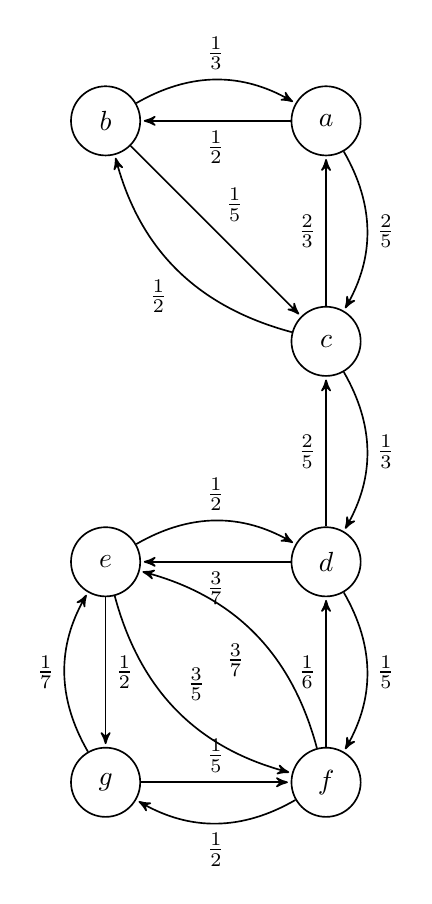
\begin{tikzpicture}[->,>=stealth',shorten >=1pt,auto,node distance=2.8cm,
                    semithick]
  \tikzstyle{every state}=[fill=none,draw=black,text=black]

  \node[state]         (A)                    {$a$};
  \node[state]         (B) [left of=A]        {$b$};
  \node[state]         (C) [below of=A]       {$c$};
  \node[state]         (D) [below of=C] {$d$};
  \node[state]         (E) [left of=D]  {$e$};
  \node[state]         (F) [below of=D] {$f$};
  \node[state]         (G) [below of=E]      {$g$};

  \path (A) edge             node {$\frac{1}{2}$} (B)
            edge  [bend left]           node {$\frac{2}{5}$} (C)
        (B) edge  [bend left]            node {$\frac{1}{3}$} (A)
            edge              node {$\frac{1}{5}$} (C)
        (C) edge              node {$\frac{2}{3}$} (A)
            edge  [bend left]            node {$\frac{1}{2}$} (B)
            edge  [bend left]            node {$\frac{1}{3}$} (D)
        (D) edge              node {$\frac{2}{5}$} (C)
            edge              node {$\frac{3}{7}$} (E)
            edge  [bend left]          node {$\frac{1}{5}$} (F)
        (E) edge  [bend left]            node {$\frac{1}{2}$} (D)
            edge  [bend right]            node {$\frac{3}{5}$} (F)
            edge             node {$\frac{1}{2}$} (G)
        (F) edge              node {$\frac{1}{6}$} (D)
            edge  [bend right]            node {$\frac{3}{7}$} (E)
            edge  [bend left]            node {$\frac{1}{2}$} (G)
        (G) edge  [bend left]            node {$\frac{1}{7}$} (E)
            edge              node {$\frac{1}{5}$} (F);
\end{tikzpicture}



\paragraph{(b)}
\begin{multicols}{2}
\text{Matlab code}
\begin{verbatim}
clear all
close all
clc
P = [0 1/3 2/3 0 0 ; 
    1/2 0 1/2 0 0 ; 
    2/5 1/5 0 2/5 0;
    0 0 1/3 0 1/2 ;
    0 0 0 3/7 0 ];
I =  eye(5);
A = inv(I - P);
S = sum(A,2)
\end{verbatim}
\text{Matlab output}
\begin{verbatim}
S =

   13.6000
   13.8000
   12.0000
    7.0000
    4.0000
\end{verbatim}
\end{multicols}
\text{Hence, the expected number of steps from a to f is 13.6}\\
\bigskip\\
\text{I give up}
\end{document}
